% This file is based on the "sig-alternate.tex" V1.9 April 2009
% This file should be compiled with V2.4 of "sig-alternate.cls" April 2009

\documentclass{sig-alternate}
\usepackage{float}
\usepackage{url}
\usepackage{color}
\usepackage{enumerate}
\usepackage{balance}
\permission{}
\CopyrightYear{2014}

\begin{document}

\title{Solving Partial Differential Equations with the use of Haskell and Parallelism}
\numberofauthors{1}
\author{
\alignauthor
Ryan Vogt
}
\date{1 Augest 2014}
\maketitle
\begin{abstract}
Partial Differential Equations are slowly but surely becoming one of the top tier areas of mathematics. The use of Partial Differential Equations are used in multiple settings such as Science, Business and Engineering. Many mathematicians have worked tirelessly in order to find methods to obtain analytical solutions to these problems. Some have found solution techniques for subsets of problems, however for the majority of problems they must be solved numerically. In this paper, there will be an introduction of solving a specific case of parabolic Partial Differential Equations, that being the heat equation. An implementation of such a program in Haskell to solve this problem will be explored in two cases. The first being able to run on a single core processor, while the other being able to work with multiple cores. Comparison between the two will be shown, and the introduction to what parallelism and Haskell can offer to solve more complex families of Partial Differential Equations. 

\end{abstract}

\section{Haskell Parallelism}
\label{overview}

Haskell lives in the class of functional languages, as a result, answers to problems are found with the use of recursion. With this perspective on computing, problems that have a easily recursive feel to them, such as solving Partial Differential Equations on boundaries is an excellent application of Haskell. However with the use of parallelism, problems that are more difficult to solve, such are Partial Differential Equations that are not of the first fundamental form, can be divided without of the fear of other divisions to solve small parts of a Partial Differential Equation on its boundary then bring the solution together when it finishes.

\section{Heat Equation Intoduction}
\label{Heq}

The general problem is presented as follows:
\[ \frac{\partial \phi}{\partial t}= \alpha^2 \frac{\partial^2 \phi}{\partial x^2} \]
Assume the rod is L meters long then:
\[  \phi(0,t)=\phi_0  \] 
\[  \phi(L,t)=\phi_L  \]   
With initial heat profile on the shaft of the rod:
\[  \phi(x,0)=f_0(x)  \] 

For the interest of showing a speficic solution to this problem to solve numerically:
\[  \phi(0,t)=0  \] 
\[  \phi(L,t)=0 \]  
\[  \phi(x,0)=x^2 +5x + 5  \]

The analytical solution to this problem which will later be examined is the following:
\[  \phi(x,t)=\sum_{n=1}^{\infty} b_n sin\frac{n{\pi}x}{L}e^{{-\frac {n^2\pi^2\alpha^2} {L^2}}t} \]
where:
\[  b_n={\frac {2} {L}}\int \limits_0^L {f(x)sin \frac{n{\pi}x}{L} dx} \] 


\section{Forward Time Center Space Method}
\label{FTCSP}
Even though the analytical solution can be found to this problem, this problem to a two dimensional problem would be more difficult. However numerical methods have been developed. There are specific methods for parabolic Partial Differential Equations, but for simplicity of implimentation and writting this paper, these will not be explored. However a general approach used is finite difference method. The idea is writting derivatives in terms of the solution function itself. The finite difference equations will be different based on the Partial Differential Equation and can be manipulated into different schemes of algorithms however, the one being explored will be Forward Time Center Space method. 

The basic form of this is decribed as followed

\[  \phi(x_i,y_{j+1})= \phi(x_i,y_j) + \alpha \frac {\bigtriangleup t} {{\bigtriangleup x}^2}(\phi(x_{i+1},y_j) -2\phi(x_i,y_m) + \phi(x_{i-1},y_m)) \] 
As a result time steps can be taken in order to solve the Partial Differential Equation within a boundary
\section{Implementation on a Single Core}
\label{Implementation}
The main idea on a single core is simple. Take a grid, break it into delta x and delta t. For each x, find the solution at t+1 for that x, then continue on until the last x is reached in the interval. When that point is reached go up a delta t. Continue this process until delta t reached the end of the interval, then return the solution. The implementation in this paper was written in Haskell, after a point on the Partial Differential Equation surface is solved for a recursive step is taken for each x, when there are no more xs, then a recursive step is taken on the ts to increment the time step by delta t, when there are no more solutions to be found, that is that t is at the end of the interval, then a list of tuples in the form of (x,y,z) are returned and a surface is plotted. 

As a result the following solution surfaces are generated going from left to right in refinement. 






\section{Implementation in Parallel }
\label{implementationf}
The idea is the same as the Single Core implementation. However in this case some things are different. When solving the Partial Differential Equation on a line, there is no asking for the solution then recurs, instead spawn a thread to find the solution which has an ID and continue to create more threads. When done with  spawning all threads on a line,  then it is possible to go through a list that contains the IDS and then retrieve them. This is done with the Par monad. The idea of the Par monad is to open up threads with spawn, then come back later and ask for the answer. Multiple threads can be spawned at one time and getting the threads is a simple command. 

With this implementation  the following solutions are gained.


\section{Differences Between Implementations - Evaluation of More Complex Systems}
\label{diff}
When comparing methods, the results do not speak to what is gained with parallel method. From above, the first plot even though they are exactly the same took different times. Both took 1010101 computations to reach their solution, the single core took approximately 17 minutes, while the parallel took 13. 4 minutes does not seem like a big deal, however lets explore the more refined approach. Refining the grid even more by making time steps smaller which correlated to 10101010 computations, took the single core took 3 hours and 15 minutes, while the parallel method took 1 hour 29 minutes. The difference can be seen here obviously, it is better to open threads on a very large line and wait for those answers to return rather than ask what the answer at each spot and then recurs. 

However there is even more to say, this Partial Differential Equation is in the first fundamental form, as a result convergence is rapid, however many interested Partial Differential Equations which are in the family of non linear Partial Differential Equations converge slowly, as a result it is impossible to approach to solve such a problem in Haskell numerically without the use of parallelism. Even for other cases, such as Elliptic or Hyperbolic Partial Differential Equations which converge more slowly than Parabolic will see great computation time improvements if solved in parallel on a cluster. 


\begin{figure}[h!]
    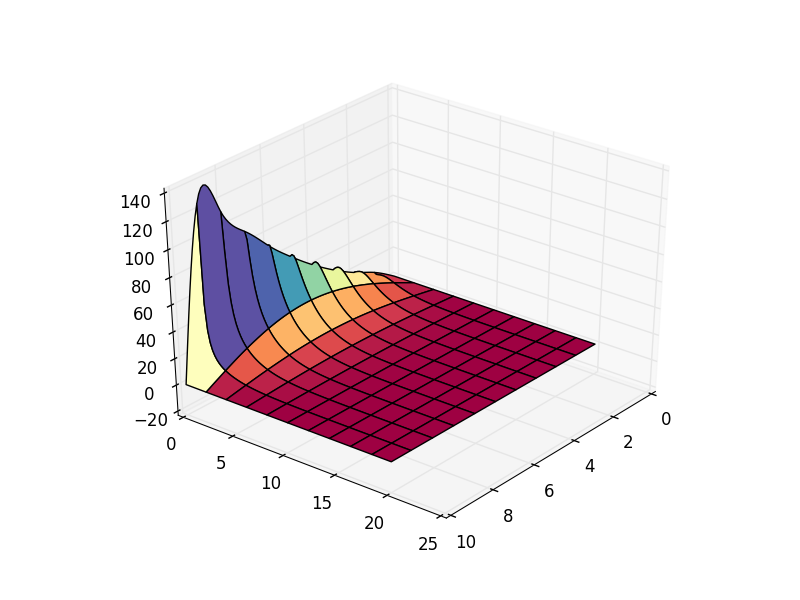
\includegraphics[scale=.5]{hhheat1}
    \caption{Took 13 minutes - parallel} 
\end{figure}

\begin{figure}[h!]
   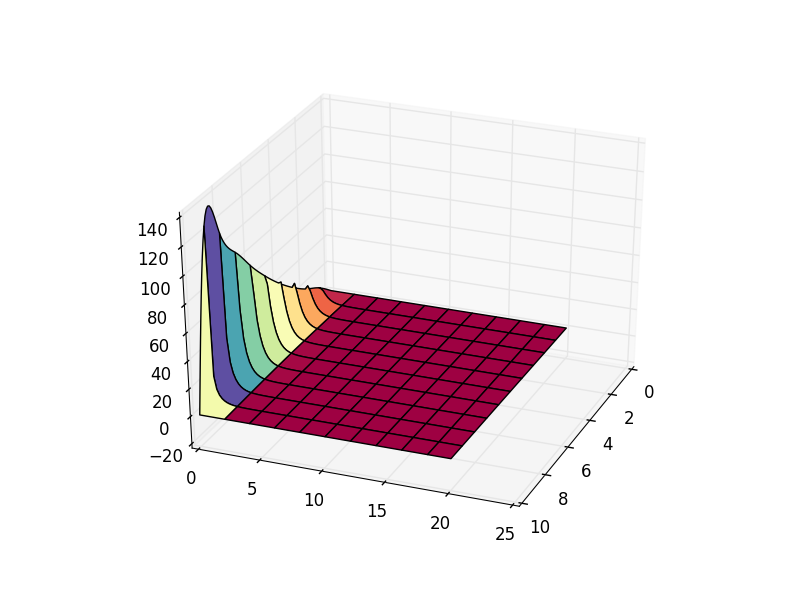
\includegraphics[scale=.5]{heat50} 
   \caption{Took 1 hours 29 Minute - parallel (refined)}
\end{figure}


\begin{figure}[h!]
    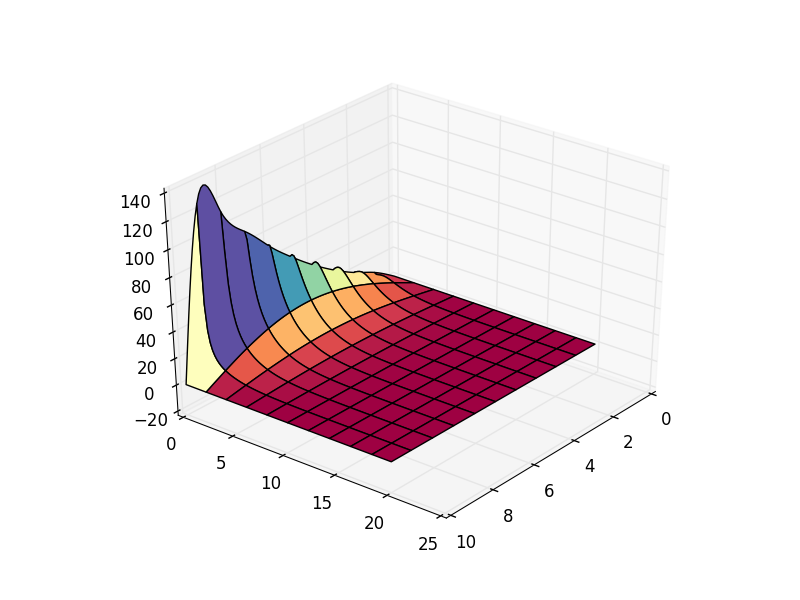
\includegraphics[scale=.5]{hhheat1} 
    \caption{Took 17 Minutes - single core}
\end{figure}

\begin{figure}[h!]
   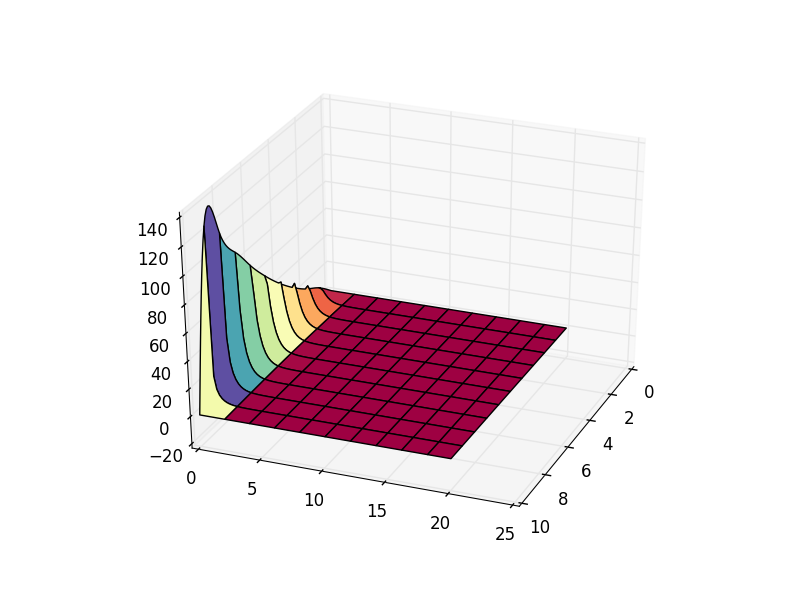
\includegraphics[scale=.5]{heat50} 
   \caption {Took 3 hours 15 Minutes - single core (refined)}
\end{figure}

% You must have a proper ".bib" file
%  and remember to run:
% latex bibtex latex latex
% to resolve all references
\balance
\end{document}








